
	\begin{enumerate}
	\item Дата собрания: 17.10.14
	\item Цель:
		\begin{itemize}
		\item Установить оставшиеся колеса, проверить подвижность робота(способность разворачиваться, заезжать на пандус и спускаться с него)
		\item Придумать(по возможности установить) конструкцию подъемника
		\end{itemize}
	\item Результаты:
		\begin{itemize}
		\item Проведя несколько пробных заездов с уже собранной конструкцией выяснилось, что робт имеет недостаточное сцепление с полем. Было решено заменить текущую колесную базу на трехколесную.
		\item Подходящих креплений для установки подъемника не нашлось. Крепления должны прочно, без люфтов, скреплять балочные элементы подъемника, при этом не создавая большого трения между ними.
		\item Для уменьшения люфтов и трения в основании конструкции были установлены выдвижные рейки(Рисунки 8, 9)
		\end{itemize}
	\item Идеи и планы:
		\begin{itemize}
		\item Установть вместо двух опорных омни-колес одно
		\item Появилась идея использовать в качестве креплений для подъемника мебельные стяжки.
		\end{itemize}
	\begin{figure} [h]
			\centering
			\begin{minipage}{0.3\linewidth}
				\includegraphics[width=35mm,height=35mm]{/!my_data/projects/pml30-psi_team/Days/17.10.14/7_1_robot}\\ Рисунок 8
			\end{minipage}
			\begin{minipage}{0.3\linewidth}
				\includegraphics[width=35mm,height=35mm]{/!my_data/projects/pml30-psi_team/Days/17.10.14/7_2_robot}\\ Рисунок 9
			\end{minipage}
			\begin{minipage}{0.3\linewidth}
				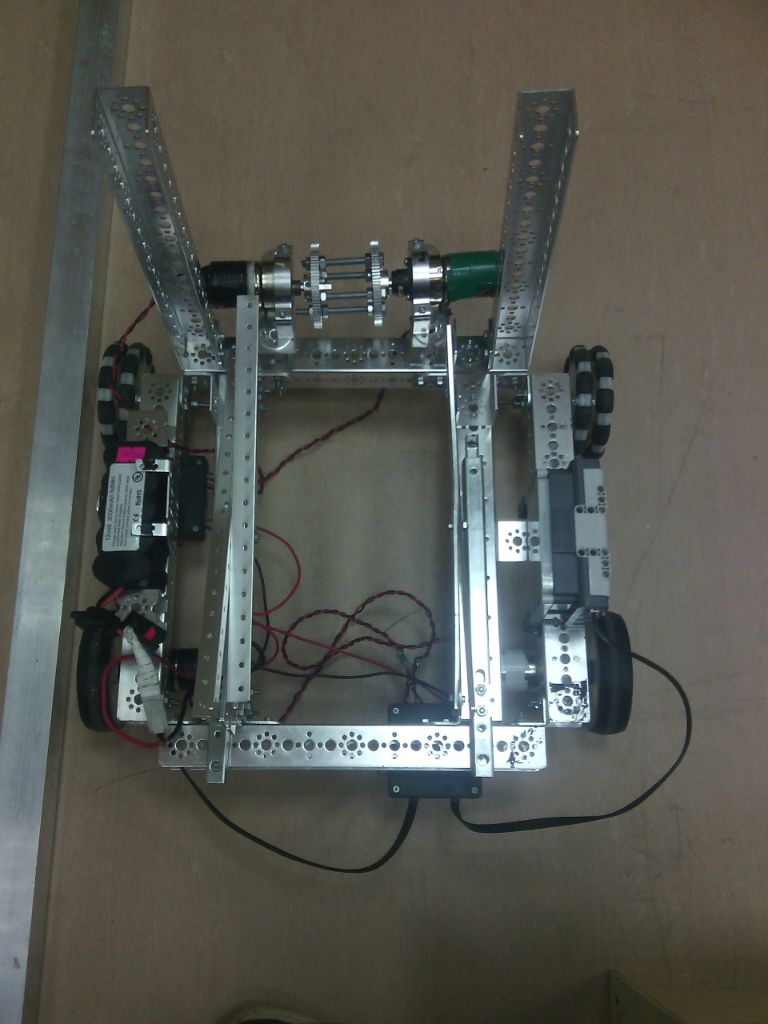
\includegraphics[width=35mm,height=35mm]{/!my_data/projects/pml30-psi_team/Days/17.10.14/7_3_robot}\\ Рисунок 10
			\end{minipage}		
	\end{figure}
	\end{enumerate}
\newpage